\documentclass[aspectratio=169]{beamer}
\usepackage[ngerman]{babel}
\usepackage{float} 
\usepackage{hyperref}
\usepackage{FiraSans}
\usepackage[font=scriptsize]{caption}
\definecolor{tudo}{HTML}{74B618}

\usetheme[sectionpage=none,titleformat frame=regular]{metropolis}
\setsansfont{Fira Sans Book}
\setbeamerfont{title}{series=\mdseries}
\setbeamerfont{frametitle}{series=\mdseries}
\setbeamercolor{background canvas}{bg=white}
\setbeamercolor{frametitle}{bg=tudo, fg=white}
\setbeamercolor{alerted text}{fg=tudo}
\setbeamercolor{progress bar}{fg=tudo}
\setbeamertemplate{bibliography item}{\insertbiblabel}

\makeatletter
\setbeamertemplate{frametitle}{
	\nointerlineskip
	\begin{beamercolorbox}[wd=\paperwidth,sep=0pt,leftskip=\metropolis@frametitle@padding,rightskip=\metropolis@frametitle@padding,]{frametitle}
		\metropolis@frametitlestrut@start
		\insertframetitle
		\nolinebreak
		\hfill
		$\mid$
		\hspace{\metropolis@frametitle@padding}
		\raisebox{-0.25mm}{
\includegraphics[height=2ex,keepaspectratio]{tud_logo_negativ.png}}
		\metropolis@frametitlestrut@end
	\end{beamercolorbox}
}
\setbeamertemplate{footline}{
	\begin{beamercolorbox}[wd=\paperwidth,sep=0pt,leftskip=\metropolis@frametitle@padding,rightskip=\metropolis@frametitle@padding,]{footline}
		\parbox{0.33\linewidth}{\vspace*{-10pt}\insertshorttitle}
		\hfill
		\parbox{0.33\linewidth}{\vspace*{-10pt}\centering\insertshortauthor}
		\hfill
		\parbox{0.33\linewidth}{\vspace*{-10pt}\hfill\insertshortdate\hspace*{10pt}\insertframenumber}
	\end{beamercolorbox}
}
\makeatother

\title[Analyse der Marsoberfläche durch Unsupervised Learning]{Kategorisieren der Marsoberfläche durch Unsupervised Learning by Backpropagation}
\author{Merlin Scholz}
\institute{TU Dortmund}
\date[20.11.2019]{20. November 2019}



\begin{document}

\frame{\titlepage}

\begin{frame}{Inhalt}
	\tableofcontents
\end{frame}

\section{Motivation}

\begin{frame}{Motivation: Neuronale Netze zur Bildsegmentierung}
\begin{columns}
	\begin{column}{.5\textwidth}
		\begin{itemize}
			\item Neuronale Netzwerke werden oft zur Bildsegmentierung genutzt
			\item Voraussetzung: Manuell erstellte Ground Truth um das Netzwerk zu trainieren
			\end{itemize}
	\end{column}
	\begin{column}{.5\textwidth}
		\begin{figure}[H]
			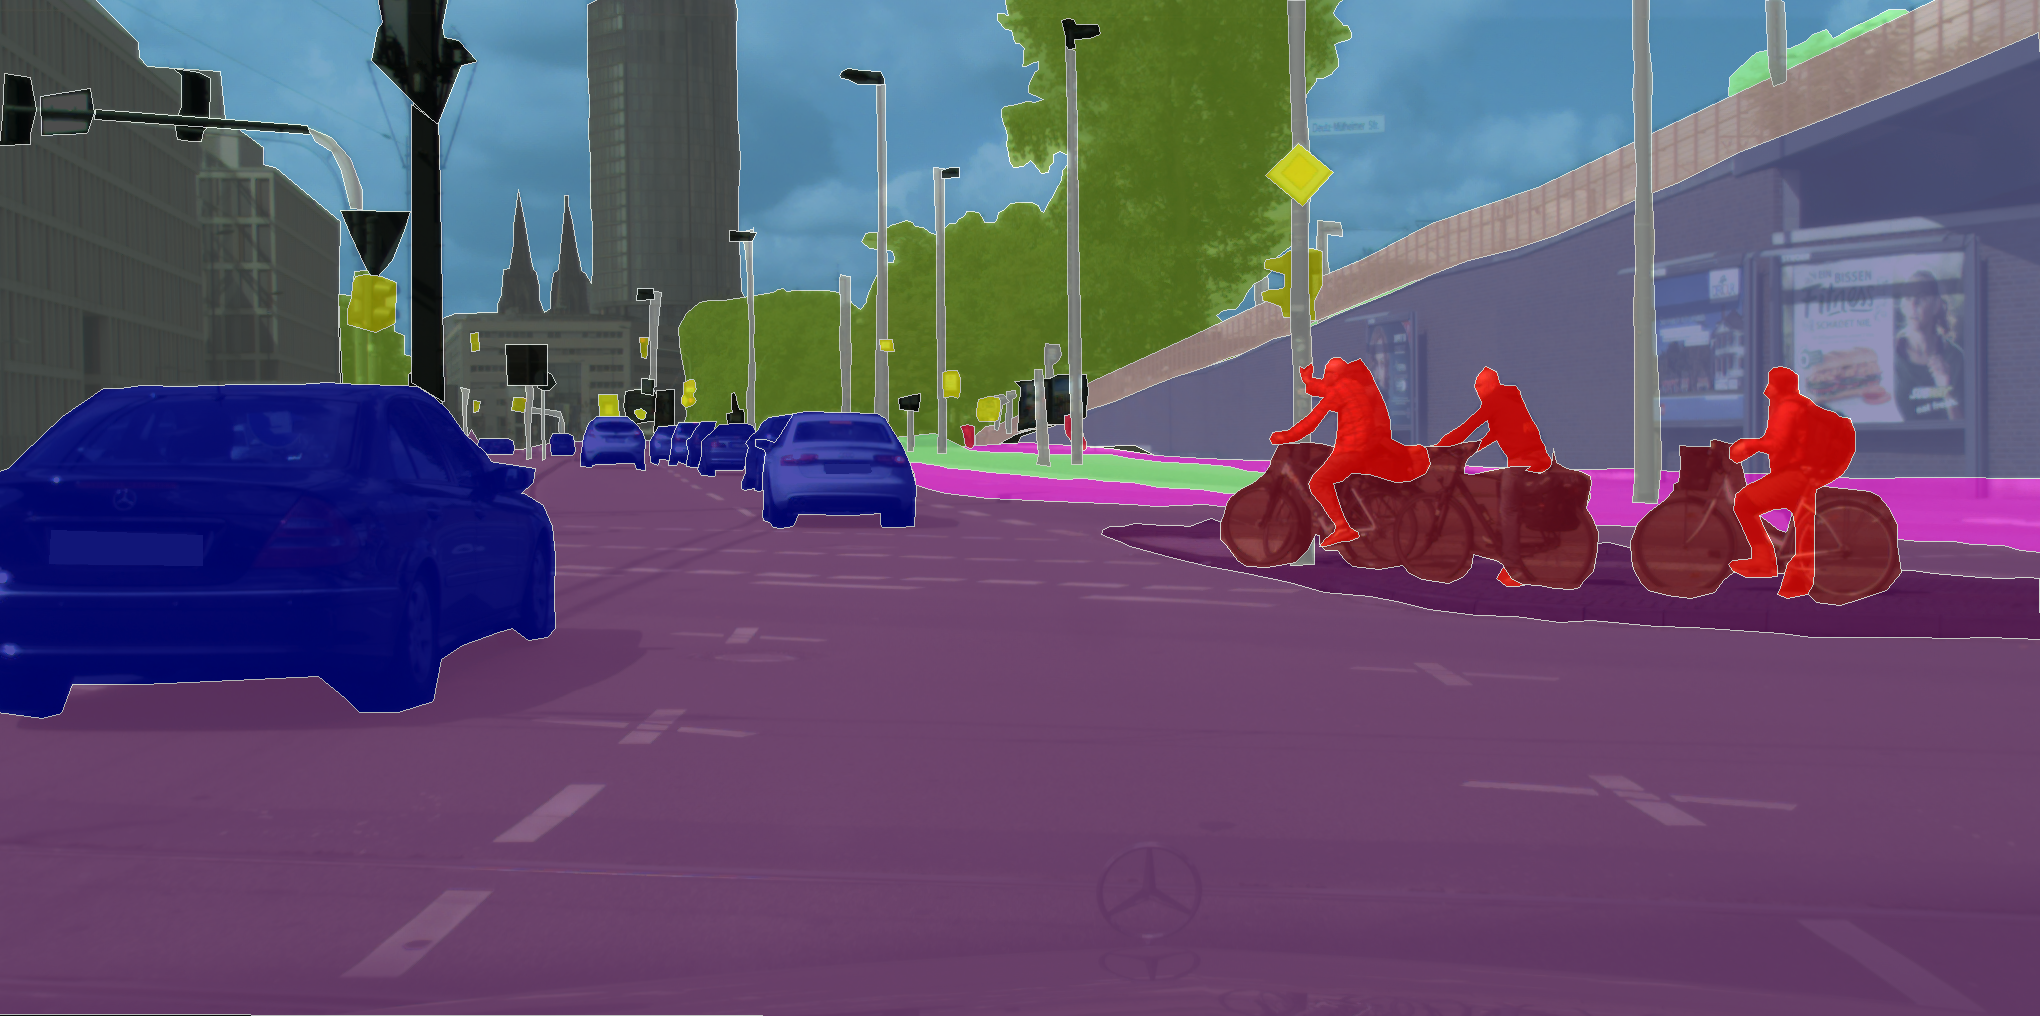
\includegraphics[width=\textwidth,keepaspectratio]{koeln00.png}
			\caption{Beispiel: CityScapes Dataset\cite{Cordts_2016_CVPR}}
		\end{figure}
	\end{column}
\end{columns}


\end{frame}

\begin{frame}{Motivation: (Fehlende) Ground Truths}
Ground Truth nicht immer vorhanden: Beispiel Marsoberfläche
\begin{itemize}
	\item Zu großer Datensatz
	\item Notwendigkeit von Experten
	\item[$\Rightarrow$] Manuelle Erstellung nicht kostengünstig oder zeiteffizient möglich
\end{itemize}
\medskip
Lösungsansatz:
\begin{itemize}
	\item Anfangs zufällige Klassifizierung durch Segmentierungsalgorithmus weiter optimieren
\end{itemize}
\end{frame}

\section{Verwandte Arbeiten}

\begin{frame}{Verwandte Arbeiten: Segmentierung nach Kanezaki\cite{kanezaki2018_unsupervised_segmentation}}
Asako Kanezaki; Unsupervised Image Segmentation by Backpropagation\cite{kanezaki2018_unsupervised_segmentation}:
\begin{columns}
	\begin{column}{.5\textwidth}
		\begin{itemize}
			\item Unüberwachtes Lernen der Segmentierung
			\item Anfangs zufällige Ergebnisse werden mit Clusteringalgorithmus vereint
			\item Zielfunktion: Softmax-Loss zwischen Ergebnis des NN und des optimierten Ergebnisses
			\item NN wird auf diese Zielfunktion hin optimiert (Backpropagation)
		\end{itemize}
	\end{column}
	\begin{column}{.5\textwidth}
		\begin{figure}
			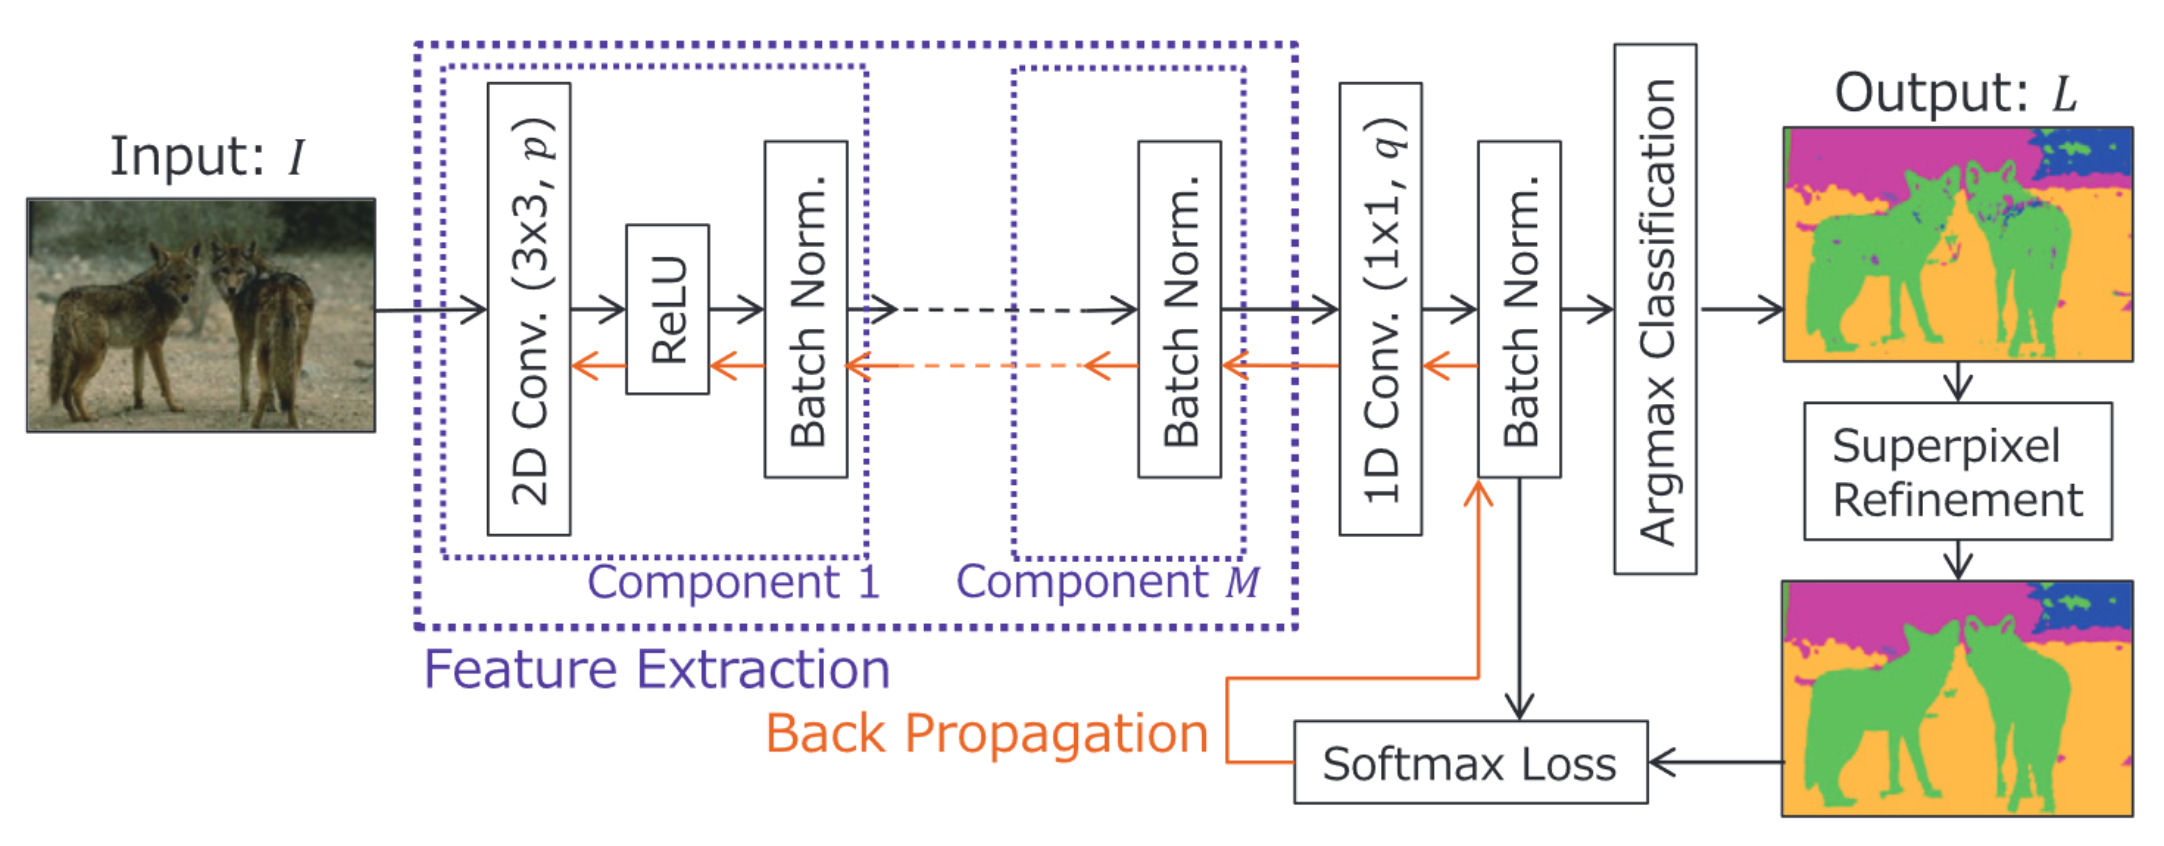
\includegraphics[width=\textwidth,keepaspectratio]{kanezaki.png}
			\caption{Vorgehensweise nach Kanezaki\cite{kanezaki2018_unsupervised_segmentation}}
		\end{figure}
	\end{column}
\end{columns}
\end{frame}

\begin{frame}{Verwandte Arbeiten: \textit{Crater Detection via CNNs}\cite{2016arXiv160100978C}}
	
\end{frame}

\section{Vorgehensweise}

\section{Referenzen}

\begin{frame}[shrink=30]{Referenzen}
	\bibliographystyle{abbrv}
	\bibliography{presentation}
\end{frame}

	
\end{document}